\documentclass[10pt, c]{beamer}
% Setup appearance:

% Standard packages
\usepackage[french]{babel}
\usepackage{times}
\usepackage[T1]{fontenc}
\usepackage{float}
\usepackage{multirow}
\usepackage{subfigure}
\usepackage{pifont}
\usepackage{tikz}
\usepackage{morewrites}
\usepackage{amsmath}
\usepackage{algorithm}
\usepackage{algorithmic}
%\usepackage{subfig}
\usetikzlibrary{arrows}
\tikzstyle{block}=[draw opacity=0.7,line width=1.4cm]
\DeclareOption{english}{\trans@use@and@alias{english}{English}}
\ProcessOptions

\mode<presentation> {
	\definecolor{bgcol}{RGB}{255,255,255}
	\definecolor{grencol}{RGB}{0,102,0}
	\definecolor{rulecol}{RGB}{3,16,67}
	\definecolor{boxtitre}{RGB}{37,45,137}
	}

  \usetheme{Warsaw}
	%\usecolortheme[named=rulecol]{structure}
	\usefonttheme[onlysmall]{structurebold}
	\usefonttheme{structureitalicserif}
	\useinnertheme{rounded}
	\useoutertheme{split}
	
	\beamertemplateshadingbackground{bgcol}{bgcol} % pour jouer sur la couleur % du fond
	\beamertemplatetransparentcovereddynamic
	\setbeamertemplate{background canvas}[vertical shading][top=white, bottom=white!60!white]
	%\setbeamercolor{normal text}{bg=rulecol,fg=black}
	%\setbeamercolor{title in head}{bg=rulecol!80,fg=bgcol}
	\setbeamercolor{title in foot}{bg=black,fg=white}
	\setbeamercolor{author in head}{bg=rulecol,fg=bgcol}
	\setbeamercolor{author in foot}{bg=black!80,fg=white}
	\setbeamercolor{section in head}{bg=black,fg=bgcol}
	\setbeamercolor{section in foot}{bg=rulecol!80,fg= bgcol}
	\setbeamercolor{subsection in head}{bg=black,fg=bgcol}
	\setbeamercolor{subsection in foot}{bg=rulecol,fg=bgcol}
	\setbeamercolor{logo}{bg=rulecol,fg=white}
	\setbeamercolor{section in head/foot}{bg=black!90,fg=white}
	\setbeamercolor{subsection in head/foot}{bg=rulecol!90,fg=white}
	\setbeamercolor{boiterouge}{bg=red!60,fg=black}
	\setbeamercolor{boiterougeB}{bg=red,fg=black}
	\setbeamercolor{boiteblanche}{bg=white,fg=black}
	\setbeamercolor{boiteverte}{bg=green,fg=black}
	\setbeamercolor{boiteblue}{bg=rulecol,fg=white}
	
	\setbeamerfont*{frametitle}{size=\normalsize}
	
	
  \setbeamertemplate{navigation symbols}{}
	\setbeamertemplate{itemize item}[square]
	\setbeamertemplate{enumerate item}[ball]
	\setbeamertemplate{itemize subitem}[triangle]
	\setbeamertemplate{itemize subsubitem}[circle]
	\logo{
\includegraphics[height=5mm]{images/logouniv.png}}
	\setbeamertemplate{footline}{
		\leavevmode%
		\hbox{\hspace*{-0.06cm}
		
		\begin{beamercolorbox}[wd=.255\paperwidth,ht=2.25ex,dp=1ex,left]{author in foot}%
			\usebeamerfont{author in head/foot}\insertshortauthor%~~(\insertshortinstitute)
		\end{beamercolorbox}%
		
		\begin{beamercolorbox}[wd=.6\paperwidth,ht=2.25ex,dp=1ex,center]{title in foot}%
			\usebeamerfont{title in head/foot}\insertshorttitle
		\end{beamercolorbox}%
		
		\begin{beamercolorbox}[wd=.145\paperwidth,ht=2.25ex,dp=1ex,right]{section in foot}%
			\usebeamerfont{logo}\textcolor[rgb]{1,0.41,0.13}{\insertshortdate{}}\hspace*{0.4em}
			\insertframenumber{} / \inserttotalframenumber
		\end{beamercolorbox}}%
		
		\vskip0pt%
	}
\renewcommand{\raggedright}{\leftskip=0pt \rightskip=0pt plus 0cm}

\title[Proposition]{}

\author[$\;\;$ TCHIO AMOUGOU Styves Daudet]{}

\date[Février 2021]{Février 2021}

%\subject{Mémoire de Master 2}
\begin{document}
\begin{frame}
\transfade
	\vspace{-0.3cm}
	\begin{figure}
		\begin{center}
		
\includegraphics[width=11cm,height=1.2cm]{images/enteteUds.PNG}
		\end{center}
	\end{figure}
	
	\begin{center}
	\tiny{\textsc{\textcolor{black}{DSCHANG SCHOOL OF SCIENCES AND TECHNOLOGY}}}\\
		\tiny{Unité de Recherche en Informatique Fondamentale, Ingénierie et  Application (URIFIA)}
	\end{center}
	\vspace{0.05cm}
\fcolorbox{boxtitre}{boxtitre}{\parbox{1\linewidth}{

\vspace{-0.3cm}
\begin{center}

\vspace{0.05cm}
 \textcolor{bgcol}{PROPOSITION}

%\vspace{0.1cm}
\end{center}

\vspace{-0.1cm}
}}
\begin{center}
\fcolorbox{bgcol}{bgcol}{
\parbox{1\linewidth}{
\begin{center}
\vspace{-0.5cm}
\footnotesize Présenté par :\\ \textbf{\textcolor{boxtitre}{ TCHIO AMOUGOU Styves daudet}} \\
\scriptsize{\textit{Matricule : CM-UDS-14SCI0251}}\\
 \tiny{\textit{Licencié en Informatique Fondamentale}}\\
 \vspace{0.3cm}
				\scriptsize{\textit{Sous la direction de }}\\
				\scriptsize{\textbf{Dr BOMGNI ALAIN Bertrand} }\\
								\tiny{(\textit{Chargé de Cours, Université de Dschang})}\\
				\end{center}
}}
\end{center}
\end{frame}

\begin{frame}{\scriptsize Sommaire}
\transwipe
\scriptsize
  \tableofcontents
\end{frame}

\section{Déclarations}
%% definitions de la virtualisation 
	\setbeamercovered{invisible}
		\begin{frame}{Déclarations}
		\transwipe
	
		\vspace{-0.25cm}
				 \begin{itemize}
				 \item $i$ = indice du Noeud i;
			 	 \item $L_{i} = $ Liste des voisins du Noeud i;
                 \item $N_{i} = \vert L_{i} \vert = $ Nombre de listes de
                 voisins du Noeud i ;
                 \item $M_{i} = $ Mémoire du noeud i:
                 \item $M_{ri} = $ Mémoire restante du noeud i;
                 \item $M_{mi} = $ Mémoire supplémentaire requise par le Noeud i
                 \item $Sawp_{i} =$ Mémoire swap du  Noeud i;
                 \item $T_{i,j} = $ Taille de la liste des voisins du noeud j voisin du noeud i;
                 \item $IN_i$ = Noeud de stockage probable;
			 	\end{itemize}
		\end{frame}
		\begin{frame}{Déclarations}
	        \begin{itemize}
	             \item $M = $ la Mémoire nécessaire pour l'exécution du protocole;\\ on a: $M = \sum_{i}\sum_{i}T_{i,j}$
	             \item $IN_{i} = -1 $ si le noeud i n'a pas besoin d'espace supplémentaire.
	        \end{itemize}
	    \end{frame}
		
	
%% avantage de la virtualisation	
\section{Conditions}
	\setbeamercovered{invisible}
		\begin{frame}{Conditions}
			\transwipe
			\vspace{-0.25cm}
		Pour pouvoir exécuter le protocole de formation de clique il faut: 
    \begin{itemize}
        \item $\sum_{i}M_{ri} > M$
        \item pour tout Noeud i du réseau, 
        \begin{itemize}
            \item $\sum_{j}\sum_{k}T_{j,k} < \sum_{j}M_{rj}$, $j\in{L_{i} +\{i\}} $ et $k \in{L_{j}}$
        \end{itemize}
    \end{itemize}
\end{frame}
\section{Définitions}
    \subsection{Notion de supériorité}
        \begin{frame}{Notion de supériorité}
            Pour comparer les  différents nœuds, nous définissons une relation " $>^\alpha$" sur les noeuds comme suit:\\
            \vspace{5mm}
            \textbf{Définition: }  $ i >^{\alpha} j$ si et seulement si:
            \begin{itemize}
                \item $M_{i} > M_{j}$ ou
                \item $M_{i} = M_{j}$ et $i > j$
            \end{itemize}
        \end{frame}
\section{Partage de la mémoire virtuelle distribuée}
    \subsection{Choix des noeuds de stockage}
        \subsubsection{Noeud en manque de mémoire}
        	\begin{frame}{}
        	    Pour tout noeud i du réseau en manque de mémoire;
        	    \begin{itemize}
        	        \item   $\forall j \in L_i$ avec $M_{mj} >0$, $M_{rj} = 0$ et $j>^{\alpha} i$.
        	        \begin{itemize}
        	            \item si la différence entre la mémoire restant de $INi$ et la mémoire manquante de j est positive.\\
        	            $M_{rIN_{i}} - M_{mj} >0$ 
        	            \begin{itemize}
        	                \item alors la mémoire restante de INi est réduit de la mémoire manquante de j  $M_{rIN_{i}} :=M_{rIN_{i}} - M_{mj}$ 
        	            \end{itemize}
        	            \item sinon la mémoire restante de $IN_i$ passe a zéro.\\$ M_{rIN_{i}}:=0$
        	        \end{itemize}
        	        \item ce premier calcul permet au noeud i de vérifier si les noeuds avec qui il est en conflit et qui sont supérieur lui peuvent tous stocker leur données sur le noeud $IN_i$. 
        	       \item si tous les noeuds supérieur a i peuvent stocker leurs données sur $IN_i$, le noeud i vérifie s'il reste de l'espace sur le Noeud $IN_i$.
        	    \end{itemize}
        	\end{frame}
        	\begin{frame}{}
        	    \begin{itemize}
        	    \item SI la mémoire restante de $IN_i$ est positive,$ M_{rIN_{i}}>0$ 
        	    \begin{itemize}
        	        \item Si la différence entre la mémoire restant de $INi$ et la mémoire manquante de i est positive.\\
        	            $M_{rIN_{i}} - M_{mi} >0$.
        	            \begin{itemize}
        	                \item le noeud i considère $IN_i$ comme noeud de stockage.
        	            \end{itemize}
        	       \item Sinon
        	             \begin{itemize}
                          \item la mémoire manquante du noeud i est réduit du reste de mémoire de $IN_i$. $M_{mi} = M_{mi} - M_{rIN_i}$,
                          \item $IN_i = $ noeud second de la mémoire virtuelle
                     \end{itemize}
        	    \end{itemize}
        	    \end{itemize}
        	\end{frame}
            \begin{frame}{}
                \begin{itemize}
                \item[]\begin{itemize}
                     \item Dans les cas où le noeud i ne peut stocker aucune de ses listes sur le noeud $IN_i$
                     \begin{itemize}
                         \item le noeud i retire le noeud $IN_i$ de sa mémoire virtuelle. 
                        \item $IN_i = $ noeud second de la mémoire virtuelle
                     \end{itemize}
                \end{itemize}
                \end{itemize}
            \end{frame}
            \begin{frame}{programme}
                \begin{algorithm}[H]
                    \caption{Choix des noeuds de stockages}
                    \begin{algorithmic}
                        \STATE $M_{Vi} = \{ j \in L_i | M_{ri} > 0 \}$ classées par ordre décroissant.
                        \STATE $S_{i} = \{ j \in L_i | M_{mi} >0$ et $j >^{\alpha} i \} $ classées par ordre décroissant.
                        \WHILE{$M_{rIN_{i}} > 0 $ et $S_i \neq \emptyset$}
                        \IF{ $M_{rIN_{i}} - M_{mj} >0$ }
                        \STATE $ M_{rIN_{i}} \leftarrow M_{rIN_{i}} - M_{mj}$
                        \STATE $ S_i \leftarrow S_i - {j}$
                        \ENDIF
                        \ENDWHILE
                        \IF{$M_{rIN_{i}} > 0$}
                            \IF{$M_{rIN_{i}} - M_{mi}<0$}
                                  \STATE $ M_{mi} \leftarrow M_{mi} - M_{rIN_{i}}$
                                  \STATE $IN_i \leftarrow M_{vi}[1]$
                            \ENDIF
                        \ENDIF
                    \end{algorithmic}
                \end{algorithm}
            \end{frame}
        \subsubsection{Noeud avec surplus de mémoire}
            \begin{frame}{}
        	    Pour tout noeud i du réseau avec un reste de mémoire:
        	    \begin{itemize}
        	    \item $S_p = \emptyset$ (Ensemble des noeuds dont i doit stocker les listes)
        	        \item   $\forall j \in L_i$ avec $M_{mj} >0$, $M_{rj} = 0$ et $IN_j = i$.
        	        \begin{itemize}
        	            \item si la différence entre la mémoire restant de $i$ est positive.\\
        	            $M_{ri}>0$ 
        	            \begin{itemize}
        	                \item alors la mémoire restante de i est réduit de la mémoire manquante de j  $M_{ri} :=M_{ri} - M_{mj}$
        	                \item $S_p = S_p \cup \{j\}$
        	            \end{itemize}
        	            \item sinon la mémoire restante de i passe a zéro.$ M_{ri}:=0$
        	        \end{itemize}
        	        \item Ce premier calcul permet au noeud i de déterminer les noeuds voisin qui ont un manque de mémoire et dont il peut satisfaire leur demande de stockage. 
        	    \end{itemize}
        	\end{frame}
        	 \begin{frame}{programme}
                \begin{algorithm}[H]
                    \caption{Recherche des noeuds a satisfaire}
                    \begin{algorithmic}
                        \STATE $S_p = \emptyset$ (Ensemble des noeuds dont i doit stocker les listes)
                        \STATE $S_{i} = \{ j \in L_i | M_{mi} >0$ et $IN_j = i \} $ classées par ordre décroissant.
                        \FOR{ $ j \in S_i$}
                            \IF{ $M_{rIN_{i}} >0$ }
                                \STATE $ M_{rIN_{i}} \leftarrow M_{rIN_{i}} - M_{mj}$
                                \STATE $ S_p \leftarrow S_p \cup \{j\}$
                            \ELSE 
                                \STATE Break
                            \ENDIF
                        \ENDFOR
                    \end{algorithmic}
                \end{algorithm}
            \end{frame}
    \subsection{Gestion des conflits}
    \subsubsection{Envoi des demandes}
        	\begin{frame}{Noeud en manque de mémoire}
        	    \begin{itemize}
        	        \item Tous les noeuds en manque de mémoire qui ont changé de $IN_i$ font une demande de $M_{mi}$ a leur nouveau $IN_i$
        	    \end{itemize}
        	\end{frame}
    \subsubsection{Traitement des demandes}
        	\begin{frame}{Noeud avec surplus de mémoire}
        	    \begin{itemize}
        	        \item  $S_d = \emptyset$ (ensemble des noeuds dont i peut satisfaire les demandes)
        	        \item   $\forall j \in L_i$ avec $M_{mj} >0$, $M_{rj} = 0$,  a reçu un demande de $M_{dj}$.
        	        \begin{itemize}
        	            \item si la différence entre la mémoire restant de $i$ et la mémoire demandée par j est positive.\\
        	            $M_{ri} - M_{dj}>0$ 
        	            \begin{itemize}
        	                \item alors la mémoire restante de i est réduit de la mémoire manquante de j  $M_{ri} :=M_{ri} - M_{dj}$
        	                \item $S_d = S_d \cup \{j\}$
        	            \end{itemize}
        	            \item sinon break
        	        \end{itemize}
        	    \end{itemize}
        	\end{frame}
        	 \begin{frame}{Traitement des demandes}
                \begin{algorithm}[H]
                    \caption{Traitement des demandes}
                    \begin{algorithmic}
                        \STATE   $S_d = \emptyset$ (ensemble des noeuds dont i peut satisfaire les demandes)
                        \STATE $S_{i} = \{ j \in L_i | M_{mi} >0$ et $M_{dj} > 0 \} $ classées par ordre décroissant.
                        \FOR{ $ j \in S_i$}
                            \IF{ $M_{rIN_{i}} >0$ }
                                \STATE $ M_{rIN_{i}} \leftarrow M_{rIN_{i}} - M_{dj}$
                                \STATE $ S_d \leftarrow S_d \cup \{j\}$
                            \ELSE 
                                \STATE Break
                            \ENDIF
                        \ENDFOR
                    \end{algorithmic}
                \end{algorithm}
            \end{frame}
    \subsubsection{envoi des réponses}
    	    \begin{frame}{envoi des réponses}
    	        \begin{itemize}
    	             \item Pour les noeuds j qui ont fait une demande de $M_{dj}$ au noeud i,
        	            \begin{itemize}
        	                \item si $j \in S_d$ la demande est approuvée;
        	               \item sinon  envoyer une message de refus au noeud j
        	            \end{itemize}
        	              \item Quand un noeud reçoit un réponse négative a une demande,
                    \begin{itemize}
                        \item le noeud i retire le noeud a qui il a fait la demande de sa mémoire virtuelle.
                    \end{itemize}
                      \item Par contre si le noeud i ne reçoit aucune réponse il considère que sa demande a été approuvée. 
    	        \end{itemize}
    	    \end{frame}
    	    \begin{frame}{envoi des réponses}
                \begin{algorithm}[H]
                    \caption{envoi des réponses}
                    \begin{algorithmic}
                        \STATE   $S_d =$ (ensemble des noeuds dont i peut satisfaire les demandes)
                        \STATE $S_{i} = \{ j \in L_i | M_{mi} >0$ et $M_{dj} > 0 \} $ classées par ordre décroissant.
                        \FOR{ $ j \in S_i$}
                            \IF{ $j \not\in S_d$ }
                               \STATE envoyer une message de refus au noeud j
                            \ENDIF
                        \ENDFOR
                    \end{algorithmic}
                \end{algorithm}
            \end{frame}
    \subsubsection{Partage d'informations sur les mémoires restantes du réseau}
    	     \begin{frame}{Partage d'informations}
    	     \begin{itemize}
    	         \item Partage d'informations sur les mémoires restantes du réseau aux différents noeuds du réseau encore en manque de mémoire.
    	         \item Recommencer a la première phase.
    	     \end{itemize}
    	 \end{frame}
    \subsection{Remplissage de la table des pages}
    	 \begin{frame}{Remplissage de la table des pages}
    	  a la fin de chaque calcul, les mappeurs synchronise les différentes table de pages. pour que chaque noeuds ai les informations complètent sur tout les endroits ou il doit stocker ses données. 
    	 \end{frame}
    	 \begin{frame}{Remplissage de la table des pages}
            \begin{algorithm}[H]
                \caption{Synchronisation des tables des pages}
                \begin{algorithmic}
                    \STATE   $S_d =$ Ensemble des noeuds dont i peut satisfaire les demandes.
                    \STATE $S_p =$ Ensemble des noeuds dont i doit stocker les listes.
                    \STATE index = 0
                    \FOR{ $ j \in S_p$}
                        \FOR{$k = 0; k < M_{mj}/T ; k++$}
                            \STATE $index \leftarrow index + k$
                            \STATE $Tap_i[index].Owner \leftarrow j$
                        \ENDFOR
                        \STATE envoyer($Tap_i[index -k ]$ a $Tap_i[index ] $ au noeud j)
                    \ENDFOR
                    \FOR{ $ j \in S_d$}
                        \FOR{$k = 0; k < M_{dj}/T ; k++$}
                            \STATE $index \leftarrow index + k$
                            \STATE $Tap_i[index].Owner \leftarrow j$
                        \ENDFOR
                        \STATE envoyer($Tap_i[index -k ]$ a $Tap_i[index ] $ au noeud j)
                    \ENDFOR
                \end{algorithmic}
            \end{algorithm}
        \end{frame}
    \section{Théorème}
    	 \begin{frame}{Théorème}
    	    Cette phase de calcul peut s'exécuter au maximum d fois avec d = dégrée le plus haut du réseau.  \\
    	    \vspace{2mm}
    	    \textbf{Preuve:} \\
    	     \vspace{2mm}
    	    Soit un réseau de N noeuds avec D le dégrée haut du réseau .\\
    	    Soit i un noeud en manque de mémoire avec $|L_i| = $ dégrée du noeud i. \\
    	    soit $M_{vi} = \{j \in |L_i| | M_{ri} >0 et M_{mi} = 0\}$
    	    \\
    	    Le noeud i peut donc faire au maximum  $|M_{vi}|$ demande. car si la demande de i a $j \in M_{vi}$ est rejeté alors $|M_{vi}|:=|M_{vi}| - \{j\}$; et i retirée j de sa mémoire virtuelle. Dans le cas contraire, le noeud i n'est plus éligible a la prochaine phase de calcul.
    	 \end{frame}
    	 \begin{frame}{Théorème}
            Donc le noeud i peut participe au maximum a $|M_{vi}|$ phases de calcul.\\ 
            $|M_{vi}| < |L_{i}| \leq D$ .
            D'où Cette étape de calcul peut se faire au maximum d fois.
    	 \end{frame}
\section{Exemple}
	\begin{frame}{Réseau}
	    \begin{figure}
        \centering
       	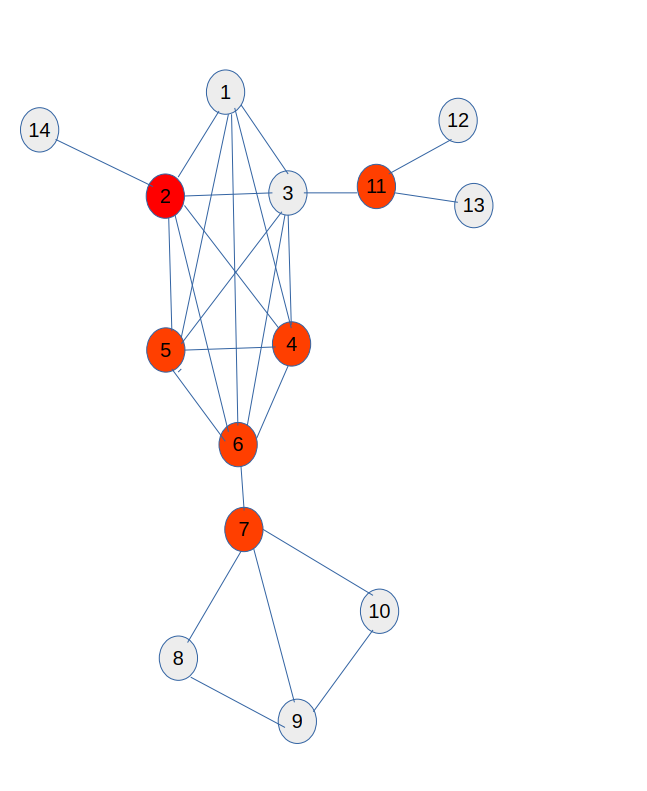
\includegraphics[width=11cm,height=7cm]{images/ExampleR.PNG}
    \end{figure}
	\end{frame}
    \begin{frame}{Informations sur les noeuds}
         \begin{figure}
        \centering
       	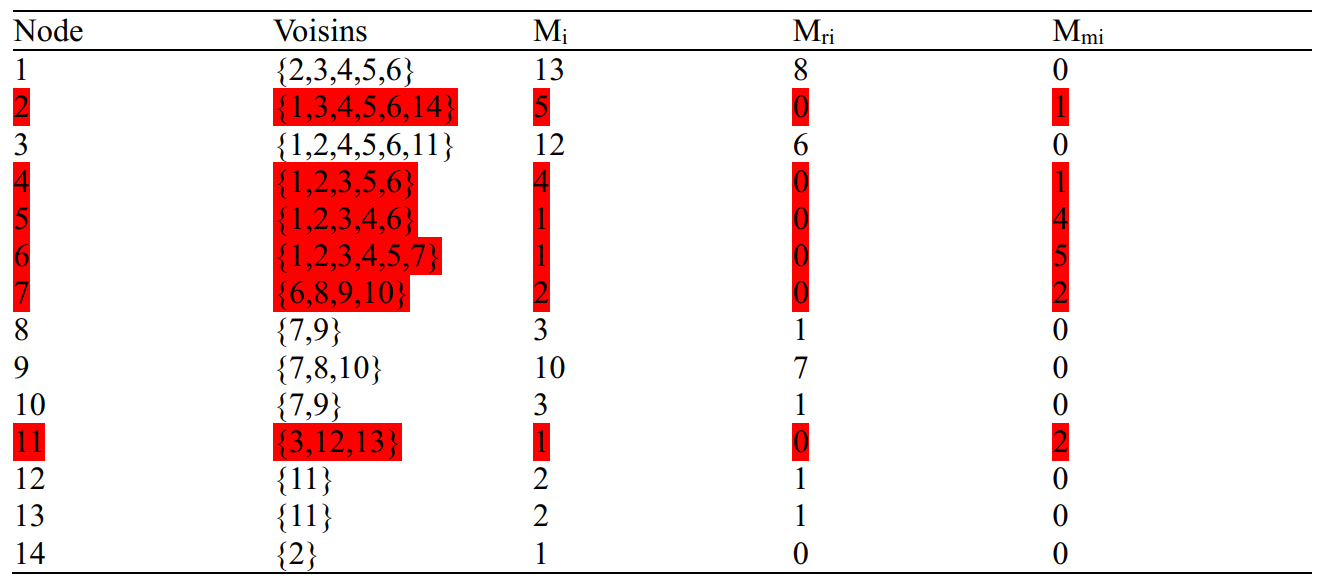
\includegraphics[width=11cm,height=7cm]{images/ExampleTable.PNG}
    \end{figure}        
    \end{frame}
     \begin{frame}{Informations sur les noeuds}
         \begin{figure}
        \centering
       	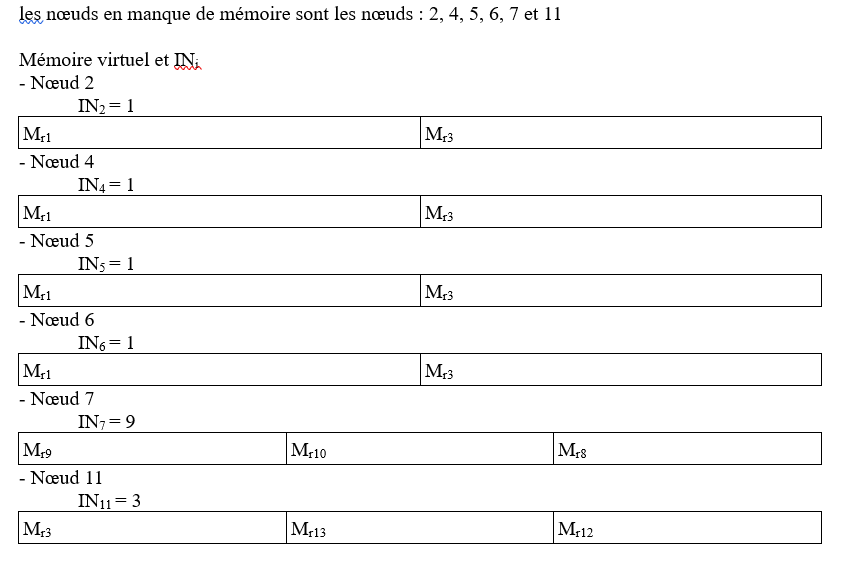
\includegraphics[width=11cm,height=7cm]{images/templateMemoryexample.PNG}
    \end{figure}       
    \end{frame}
    \begin{frame}{Pour le Noeud 2}
    \begin{itemize}
        \item  $L_2 = \{1,3,4,5,6,14\}$, Les voisins du noeud 2 en manque de mémoire avec le même $IN_2 = 1$ sont:  $\{4,5,6\}$
        \item en classant les noeuds par ordre de grandeur on: 6 > 5> 4> 2.
        \item La mémoire du noeud 1 ne peut satisfaire que 6 et 5.
        \item  donc le noeud 2 fait une demande 1T au noeud 3 et retire le noeud 1 de sa mémoire virtuelle
    \end{itemize}
    \end{frame}
    \begin{frame}{Pour le Noeud 4}
    \begin{itemize}
        \item  $L_4 = \{1,2,3,5,6\}$, Les voisins du noeud 4 en manque de mémoire avec le même $IN_4= 1$ sont:  $\{2,4,5,6\}$
        \item en classant les noeuds par ordre de grandeur on: 6 > 5> 4> 2.
        \item La mémoire du noeud 1 ne peut satisfaire que 6 et 5.
        \item  donc le noeud 4 fait une demande 1T au noeud 3 et retire le noeud 1 de sa mémoire virtuelle
    \end{itemize}
    \end{frame}
     \begin{frame}{Pour le Noeud 5}
    \begin{itemize}
        \item  $L_5 = \{1,2,3,4,6\}$, Les voisins du noeud 5 en manque de mémoire avec le même $IN_5 = 1$ sont:  $\{2,4,6\}$
        \item en classant les noeuds par ordre de grandeur on: $6 > 5> 4> 2.$
        \item La mémoire du noeud 1 ne peut satisfaire que 6 et il reste 3T au noeud 1 
        \item le noeud 5 fait une demande de 3T au noeud 1 et de 1T au noeud 3
    \end{itemize}
    \end{frame}
    \begin{frame}{Pour le Noeud 6}
    \begin{itemize}
        \item  $L_6 = \{1,2,3,4,5,7\}$, Les voisins du noeud 6 en manque de mémoire avec le même $IN_6 = 1$ sont:  $\{2,4,6\}$
        \item en classant les noeuds par ordre de grandeur on:$ 6 > 5> 4> 2.$
        \item noeud 6 est le noeud maximal 
        \item La mémoire du noeud 1 ne peut satisfaire le noeud 6
        \item le noeud 6 fait une demande de 5T au noeud 1.
    \end{itemize}
    \end{frame}
    \begin{frame}{Pour le Noeud 7}
    \begin{itemize}
        \item  $L_7 = \{6,8,9,10\}$, le noeud 7 n'est en conflit avec aucun de ses voisins. 
        \item La mémoire du noeud 9 peut satisfaire le noeud 7
        \item le noeud 7 fait une demande de 2T au noeud 9.
    \end{itemize}
    \end{frame}
    \begin{frame}{Pour le Noeud 11}
    \begin{itemize}
        \item  $L_{11} = \{3,12,13\}$, le noeud 11 n'est en conflit avec aucun de ses voisins. 
        \item La mémoire du noeud 3 peut satisfaire le noeud 11
        \item le noeud 11 fait une demande de 2T au noeud 3.
    \end{itemize}
    \end{frame}
     \begin{frame}{Pour le Noeud 3}
    \begin{itemize}
        \item  $S_{p} = \{11\}$, et  $S_{d} = \{5,4,2\}$
        \item La mémoire du noeud 3  satisfaire les noeuds 5,4,2 et 11
    \end{itemize}
    \end{frame}
    \begin{frame}{Pour le Noeud 1}
    \begin{itemize}
        \item  $S_{p} = \{6,5\}$, et  $S_{d} = \emptyset$
        \item La mémoire du noeud 1  satisfaire les demandes des noeuds 5,4,2 et 11
    \end{itemize}
    \end{frame}
     \begin{frame}{Pour le Noeud 9}
    \begin{itemize}
        \item  $S_{p} = \{7\}$, et  $S_{d} = \emptyset$
        \item La mémoire du noeud 1  satisfaire les demandes des noeuds 7
    \end{itemize}
    \end{frame}
%\bibliographystyle{apacite} 
%\bibliography{References/references}

%\subject{Mémoire de Master 2}
\begin{frame}
\transfade
	\vspace{-0.3cm}
	\begin{figure}
		\begin{center}
		
\includegraphics[width=11cm,height=1.2cm]{images/enteteUds.PNG}
		\end{center}
	\end{figure}
	
	\begin{center}
	\tiny{\textsc{\textcolor{black}{DSCHANG SCHOOL OF SCIENCES AND TECHNOLOGY}}}\\
		\tiny{Unité de Recherche en Informatique Fondamentale, Ingénierie et  Application (URIFIA)}
	\end{center}
	\vspace{0.05cm}
\fcolorbox{boxtitre}{boxtitre}{\parbox{1\linewidth}{

\vspace{-0.3cm}
\begin{center}

\vspace{0.05cm}
 \textcolor{bgcol}{Storage Virtualization}

%\vspace{0.1cm}
\end{center}

\vspace{-0.1cm}
}}
\begin{center}
\fcolorbox{bgcol}{bgcol}{
\parbox{1\linewidth}{
\begin{center}
\vspace{-0.5cm}
\footnotesize Présenté par :\\ \textbf{\textcolor{boxtitre}{ TCHIO AMOUGOU Styves daudet}} \\
\scriptsize{\textit{Matricule : CM-UDS-14SCI0251}}\\
 \tiny{\textit{Licencié en Informatique Fondamentale}}\\
 \vspace{0.3cm}
				\scriptsize{\textit{Sous la direction de }}\\
				\scriptsize{\textbf{Dr BOMGNI ALAIN Bertrand} }\\
								\tiny{(\textit{Chargé de Cours, Université de Dschang})}\\
				\end{center}
}}
\end{center}
\end{frame}
\end{document}